\documentclass{article}

% if you need to pass options to natbib, use, e.g.:
%     \PassOptionsToPackage{numbers, compress}{natbib}
% before loading neurips_2020

% ready for submission
%\usepackage{neurips_2020}

% to compile a preprint version, e.g., for submission to arXiv, add add the
% [preprint] option:
     \usepackage{neurips_2020}

% to compile a camera-ready version, add the [final] option, e.g.:
%     \usepackage[final]{neurips_2020}

% to avoid loading the natbib package, add option nonatbib:
 %    \usepackage[nonatbib]{neurips_2020}

\usepackage[utf8]{inputenc} % allow utf-8 input
\usepackage[T1]{fontenc}    % use 8-bit T1 fonts
\usepackage{hyperref}       % hyperlinks
\usepackage{url}            % simple URL typesetting
\usepackage{booktabs}       % professional-quality tables
\usepackage{amsfonts}       % blackboard math symbols
\usepackage{nicefrac}       % compact symbols for 1/2, etc.
\usepackage{microtype}      % microtypography
\usepackage{graphicx}

\title{Cyclist detection in aerial images}

% The \author macro works with any number of authors. There are two commands
% used to separate the names and addresses of multiple authors: \And and \AND.
%
% Using \And between authors leaves it to LaTeX to determine where to break the
% lines. Using \AND forces a line break at that point. So, if LaTeX puts 3 of 4
% authors names on the first line, and the last on the second line, try using
% \AND instead of \And before the third author name.


\author{Péter Tamás Kovács\\
team: 'zold137'\\
former members:\\
Ádám Zsolt Kővári, Soma Juhász}

\begin{document}

\maketitle



\begin{abstract}
 In this contribution, I propose an algorithm for detection of cyclists in aerial images. This task is somewhat different from the standard object recognition problems, since the bird's eye perspective prohibits direct transfer learning from datasets as eg. COCO or ImageNet. Nevertheless, a transfer learning solution is proposed but the base model is chosen with special care. The training and evaluation is performed on a dataset containing annotated pictures from Giro d'Italia 2015.  
\end{abstract}

\section{Object detection in aerial pictures}

Object detection is one of the most important branches of computer vision. Since in any realistic environment, the machine-learning agent receives visual input containing multiple objects, it is vital to be able to detect and correctly classify environmental objects to give meaningful responses to external stimuli.\\

With the rise of unmanned aerial vehicles (UAVs or 'drones') the amount of visual data captured from a bird's eye perspective is fastly growing. It is the anticipation that one day, autonomous UAVs will considerably contribute to many businesses eg. delivery or agriculture.\footnote{And sadly, military applications and surveillance.} \\

These trends call for increased attention and effort to computer vision for aerial applications. This domain is different from conventional CV applications, because the data is unlike widely adopted standard datasets (COCO, ImageNet) since everything is captured from the height. Henceforth, re-training conventional object detection architectures is one promising way to go with preserving the basic principles of modern object recognition but tailoring weights to our special needs.\\

\section{Literature survey, existing solutions}

In this section, I first give an short overview of the fundamentals of modern object recognition. In the following, I introduce the particular results of earlier investigations on which the project is based. For a very concise overview, I direct the reader to a series of blog posts that fantastically capture the main points and put the field in context.$^{\cite{weng}}$ Thank you Lilian.  

\subsection{Object detection algorithms}

The coming parts are rather standard introduction and laying the foundations for later discussion but by no means a comprehensive review of the enormous field of object detection.

\subsubsection{Preliminaries and basic notions}

The task of object detection algorithms is twofold: (i) detect objects on a given input image, (ii) classify the objects it has identified.

The solution to this task can be broken down to two parts: first, finding proposals for possible objects and then using a conventional convolutional architecture to classify proposals.\\

It is not trivial how to measure the soundness of a proposal for a Region of Interest (ROI) or actually how to represent objects inside images. In this work, we stick with the \textit{bounding box} representation, which is assigning a rectangular box to every object that is possibly the smallest box fully containing the object. Our language is obviously loose here, but at the end of the day, boxes are determined by humans annotating the images so no precise definition is possible. More advanced approaches use segmentation masks that respect the shape of objects, but here we cannot go into details.\\

For bounding boxes, a very common metric to assess the soundness of the ROI is the \textit{Intersection Over Union} (IOU) which has a pretty straightforward meaning for a ROI proposal and a ground truth box: measure the intersection's area and divide by the union's area. How ROIs are assigned to ground truth (GT) boxes can vary from implementation to implementation. A very common choice is to assign ROIs to that GT box for which the maximal IOU is attained.\\

For a given proposed region, classification is done with a CNN architecture. Unfortunately, due to scarcity of room, I cannot elaborate more on the details of how ROIs are divided into foreground and background and similar, more advanced topics. The interested reader can look it up in any competent GitHub repository.



\subsection{Architectures}

In this section, I only introduce the \textit{Faster-RCNN} architecture in detail since this is the one used in the project.\\

\subsubsection{History}

Surprisingly from the two fundamental tasks of object recognition systems, the problem of ROI proposals has been addressed earlier in a competent way. The famous \textit{Felzenszwalb algorithm} uses a graph representation of the images to basically perform clustering\footnote{Our language is loose again: this may rather be the \textit{selective search} component of the segmentation solution} on the pixels.$^{\cite{felzen}}$

The other task has been first satisfyingly tackled in the 2012 landmark AlexNet network. Blending together the two parts followed fast.$^{\cite{rcnn}, \cite{fast-rcnn}}$  

\subsubsection{Faster-RCNN}


\begin{figure}[h]
  \centering
  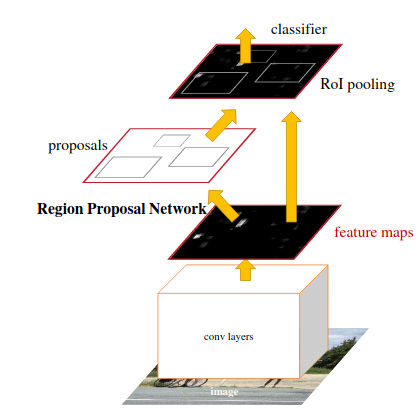
\includegraphics[scale=0.5]{fasterrcnn.png}
  \caption{The three main parts of the Faster-RCNN architecture $^{\cite{faster-rcnn}}$}
  \label{fig:faster_rcnn}
\end{figure}


This method was novel in the sense that surpassing the traditional segmentational methods, it also used a neural network architecture to generate ROI proposals. The basic sturcture of a Faster-RCNN network is depicted in figure \ref{fig:faster_rcnn}.\\

The three main parts: 

\begin{itemize}
    \item \textbf{backbone}: this part is in fact a convolutional neural network with top classification layers 'peeled off'. Its purpose is feature extraction for later stages.
    
    \item \textbf{RPN}: aka Region Proposal Network. This is the part that produces ROI proposals from the output of the backbone. Again, we cannot dive into the details but you shall look up \textit{anchor boxes} that are basically some fixed 'basic box proposals' from which the actual proposition's coordinates are determined via regression.
    
    \item \textbf{ROI head}: in this part, we basically do the classification of the proposed regions. I repeatedly stress that the above description is only a vague one, you shall look up literature.
\end{itemize}

In summary, the output of a forward pass on the network is a list of proposed boxes with the predicted labels and confidency scores for the labels. I also used a Faster-RCNN net in the project. In particular, the used model goes by the name of \verb|e2e_faster_rcnn_X_101_32x8d_FPN_1x|, you may look it up at the respective FAIR model zoo. (For more details, it is the best to refer to the config file from which the model is actually built.)

\subsubsection{More advanced networks}

In spite of being a great imporvement over its predecessors, Faster-RCNN is not the most advanced arch actually. \\

In terms of speed, there are much more competent solutions.$^{\cite{yolo}, \cite{ssd}, \cite{retinanet}}$\\

Another qualitative improvement is implemented in the \textit{Mask-RCNN} familiy where not only boxes but the very segmentation of the picture is also computed. $^{\cite{mask-rcnn}}$

\subsection{Leveraged earlier solutions}

The final solution has been built upon an earlier solution for the \textbf{VisDrone} dataset, introduced in the next section. As we had access only to limited GPU time and as being newcomers to the field, we realized that this was the way to go. The solution is due to  \textit{Oytun Ulutan} at UC Santa Barbara, and can be found under: 

\url{https://github.com/oulutan/Drone_FasterRCNN}

Fortunately, the weights of the model are also published so the transfer scenario could be implemented. We had to amend the number of classes to our specific application, so practically trimmed the the last layers of the network and replaced them with the ones in agreement with our class numbers.\\

Oytun's work is actually a fork of FAIR's \verb|maskrcnn-benchmark| repo,$^{\cite{maskrcnn}}$ under

\url{https://github.com/facebookresearch/maskrcnn-benchmark}



\section{Data sources}

As we have decided to do an UAV project, we started looking up accessible databases. Two have been found:

\begin{itemize}
    \item \textbf{VisDrone DET-2019 dataset}:$^{\cite{vdrone1},\cite{vdrone2}}$ This dataset consits of images taken by different UAVs under various conditions, eg. in urban and rural areas, under varying lightning and weather conditions, from different heigths, with few or many objects in one picture. The dataset was collected by the AISKYEYE team at Lab of Machine Learning and Data Mining, Tianjin University, China. Although the repo is unclear about licensing, we believe that the data is free to be used for research purposes.
    
    \item \textbf{MultiDrone} The public MultiDrone Dataset$^{\cite{multidr}}$ has been assembled using both pre-existing audiovisual material and newly filmed UAV shots. The dataset is curated by the Multidrone Consortium. A large subset of these data has been annotated for facilitating scientific research, in tasks such as visual detection and tracking of bicycles, football players, human crowds, etc. A dataset for bicycle detection/tracking was assembled, consisting of 3 Youtube videos\footnote{In fact, there were seven, but due to scarcity of time (the videos had to be hand-curated, see later, only three were used} (resolution: 1920 x 1080) at 25 frames per second. Annotations are not exhaustive, i.e., there may be unannotated objects in the given video frames. The license agreement allows to use only for scientific research, testing and development purposes and we aren’t authorized to put any part of the dataset on the publicly accessible Internet.

\end{itemize}

Since the input model for transfer learninig was trained on the VisDrone data, I only used the Multidrone images in the transfer learning. Due to licensing issues, I had to invent a way not to make annotations publicly available but to preserve the reproducibility of the results. The final solution was setting up a secret GitHub Gist to that I will provide access upon reasonable request.

\section{Data preparation}

The frames were fetched from YouTube. What I realised were that 

\begin{itemize}
    \item The data has to be manually curated. In fact, the videos contained (annotated) frames that were captured from the ground so showed the competitors from a totally different angle from the usual aerial view. This was remedied by watching all the relevant parts and marking the segments in which real bird's eye perspective was presented. (Part of the reasons I worked with only three videos)
    
    \item The annotations have been prepared on 1920x1080 resolution but the images have been fetched in 1280x720. Unfortunately, one of my former teammates \--- who had written the script \--- failed to notice/mention this which would have saved me a lot of time and GPU time...
\end{itemize}


\section{Utility engineering}

As there is no rose without thorn, the VisDrone project came almost with no documentation whatsoever. After correcting and extending the Dockerfile, a final version has been uploaded to the GitHub repository. With this, any interested person should be able to set up the environment on his/her device. (After PM-ing me for the code of the annotations. For detailed instructions, refer to the repository.)\\

Handling the dataset with dataloaders was only possible after writing a new module for handling the Giro images, since this is by no means a standard dataset. Interestingly, the original code did not contain any type of on the fly validation for training nor callbacks.\footnote{Or they have been hidden deliberately :) } Even more interestingly, I am not sure if Pytorch contains \textit{native} callbacks at all. (Ignite aside, since that was opted out for this project \--- I am not sure if it would have required rewriting it all.)\\

This means that I had to write these utilities \--- with reloading custom weights for the network and customizing trainable weights \--- almost from scratch. Nevertheless, it has been done since without them, it would not have been possible to do any meaningful training.\\

Finally, as for 'visible' evaluation, I also put together (mostly from other parts of the library) a pipeline that does the inference on single images and then draws the predicted boxes on top of them. 

\section{Training and evaluation}

This is actually the section where all the mentioned sufferings paid off. After having a \textit{stable} train-validation pipeline, the training was quite straightforward\footnote{Or it seems so. If you want to train your net, you must refer to the repo for the caveats. I somewhat wasted most of my time because the Visdrone weights have not been loaded properly. I only found out recently, when I haven't been able to overfit a minibatch. So for the record: it is done by the checkpointer, surprisingly.}

\begin{enumerate}
    \item Loading weights from the VisDrone project
    \item Peeling off the classification layers and replacing them with the appropriate sized layers for our problem (number of classes)
    \item Updating state dict if applicable
    \item Freezing custom layers. First, I only unfroze the newly added (so 'factory initialized') layers. In the second run, I also unfroze the whole RPN and ROI head, to attain even better convergence 
    \item Finally start training 
\end{enumerate}

\subsection{Technical details}

For every video, frames have been randomly split into train, test and validation sets with approximate ratios 0.85 : 0.10 : 0.05. This is not exact since I had to remove frames that were inappropriate for training: either bad perspective or containing unidentified objects (in the annotations, we had '-' instead of some class). 

So finally, the numbers:

\begin{table}[h]
    \centering
    \begin{tabular}{|c|c|c|c|} \hline
       video  & \textbf{giro1} & \textbf{giro4} & \textbf{giro8} \\ \hline
        train  & 2389 & 431 & 60 \\ \hline
        test &  258 & 7 & 3 \\ \hline
        \end{tabular}
        \vspace{10pt}
    \caption{Number of images in respective datasets}
    \label{tab:data}
\end{table}

I haven't included the validation numbers. This is merely because validation was not really there to assess performance precisely, but to see if the IOU values were acceptable or not (when I started experimenting they were absolutely not). To save time, I only validated on few images. 

This is kind of unfortunate practice, but I had to speed up everything because I was in acute need of time after all my teammates abandoned me and skeletons unexpectely started popping out of the closet (weight loading, having received unmatching pics to annotations, need to do hand-curating, etc.) Nevertheless, the convergence on the trainset was saturated by the end but the accuracy of predictions on the validation set was in a raising trend even when train loss stagnated.

\subsection{Evaluation}

The evaluation is based on the transfer-trained model's performance on the testsets.\\

I used two widespreadly used metrics: accuracy of predictions on the ground truth boxes and the mean recall for IOU values which I will define in the following. 

First, one defines threshold values for assessing IOU values. In our case, they were:  
[0.5000, 0.5500, 0.6000, 0.6500, 0.7000, 0.7500, 0.8000, 0.8500, 0.9000,
        0.9500]. After this, one calculates the proportion of IOU values that lie above the threshold: this gives the recall for that threshold. The mean of those values us the mean threshold. (If you are dissatisfied with this much aggregation, I totally understand, please refer to the logfiles for more details.)
        
The results are presented in table \ref{tab:data}. What we can see that the performance is satisfying for sets 1 and 8 but really bad for set 4. I hypothesize that it is due to the fact that different videos showed different conditions and the data was not of the same distribution. 

By this I mean that the notorious data featured cyclists of label 'front view' whereas cyclists are typically shown in competitions in 'back view'. Unfortunately, I haven't had time to elaborate on this issue but the probable inbalance in class distributions may be remedied.

\begin{table}[h]
    \centering
    \begin{tabular}{|c|c|c|c|} \hline
       testset  & \textbf{giro1} & \textbf{giro4} & \textbf{giro8} \\ \hline
        number of GT boxes  & 1516 & 18 & 25 \\ \hline
        accuracy &  0.81 & 0.0 & 0.80 \\ \hline
        mean recall & 0.46 & 0.03 & 0.42 \\ \hline
        \end{tabular}
        \vspace{10pt}
    \caption{Evaluation results}
    \label{tab:data}
\end{table}

\subsection{Demo}

Here, I present some impressions what I acquired while looking at predictions drawn on figures.\\

First and foremost, looking at figure \ref{fig:pred} is really sobering: it is pretty much possible that the algorithm learned to recognize the TV graphics! I also found some inconsistent behaviour (seeming mismatch between annotations and images). This must be cleared in any further project.
 
\begin{figure}[h]
    \centering
    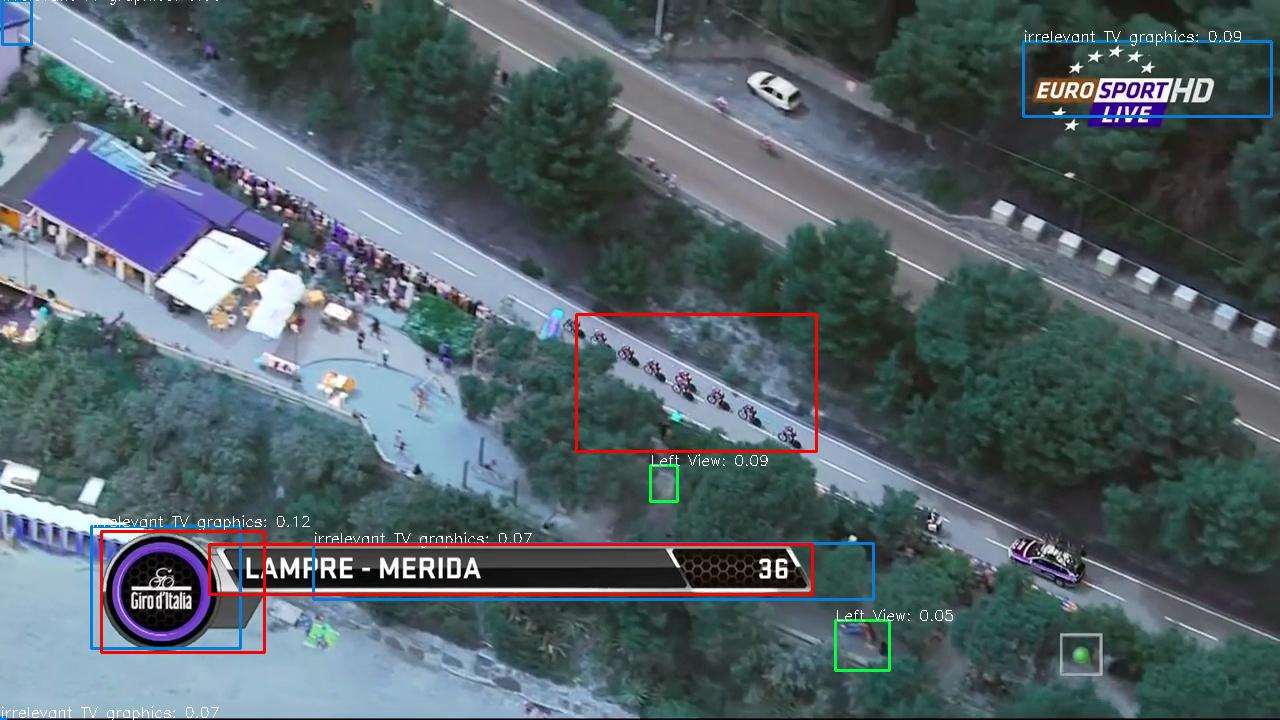
\includegraphics[scale=0.32]{pred_giro1_1336.jpg}
    \caption{Predicted boxes vs. ground truth (red)}
    \label{fig:pred}
\end{figure}

It is really hard to write down this, but the above suggests that our results are barely meaningful. In any future project, class balance (TV graphics!) shall be investigated in detail. Also, this means that the work I introduced is only making work the machinery but not yet getting acceptable results.


\section{Conclusion, plans}

To sum up, I must say that to achieve acceptable results, more training and deeper analysis of the data is indispensable. \\

It is however a fact calling for respect that I had to do the project almost totally alone while my teammates left before doing any meaningful work.

\begin{itemize}

    \item First and foremost, it shall be investigated if the annotations really match the frames. (Some results on set 'giro4' hint otherwise, but I noticed this so late that I couldn't go into much detail)

    \item Then, accuracy and IOU values shall be broken down to classes not to have dominant TV graphics or suppressed classes eg. front view
    
    \item It must be re-considered what kinds of metrics to use to assess performance we really care about 
    
\end{itemize}












\begin{thebibliography}{}
\bibitem{weng}  Lilian Weng,\\
\url{https://lilianweng.github.io/lil-log/2017/10/29/object-recognition-for-dummies-part-1.html}

\bibitem{rcnn} Ross Girshick et al. \\
Rich feature hierarchies for accurate object detection and semantic segmentation\\
\url{https://arxiv.org/abs/1311.2524}

\bibitem{fast-rcnn} Ross Girshick, \\
Fast R-CNN \\
\url{https://arxiv.org/pdf/1504.08083.pdf}

\bibitem{faster-rcnn} Shaoqing Ren et al, \\
Faster R-CNN: Towards Real-Time ObjectDetection with Region Proposal Networks \\
\url{https://arxiv.org/pdf/1506.01497.pdf}

\bibitem{mask-rcnn} Kaiming He et al,\\
Mask R-CNN\\
\url{https://arxiv.org/pdf/1703.06870.pdf}

\bibitem{yolo} Joseph Redmon et al\\
You Only Look Once:Unified, Real-Time Object Detection \\
\url{https://www.cv-foundation.org/openaccess/content_cvpr_2016/papers/Redmon_You_Only_Look_CVPR_2016_paper.pdf}

\bibitem{ssd} Wei Liu et al,\\
SSD: Single Shot MultiBox Detector\\
\url{https://arxiv.org/abs/1512.02325}

\bibitem{retinanet} Tsung-Yi Lin et al, \\
Focal Loss for Dense Object Detection\\
\url{https://arxiv.org/abs/1708.02002}

\bibitem{felzen} Pedro F. Felzenszwalb \& Daniel P. Huttenlocher \\
Efficient Graph-Based Image Segmentation \\
International Journal of Computer Vision 59, 167–181 (2004). https://doi.org/10.1023/B:VISI.0000022288.19776.77

\bibitem{vdrone1} Vision meets drones: A challenge, Zhu, Pengfei and Wen, Longyin and Bian, Xiao and Ling, Haibin and Hu, Qinghua, arXiv preprint arXiv:1804.07437, 2018

\bibitem{vdrone2} Vision Meets Drones: Past, Present and Future, Zhu, Pengfei and Wen, Longyin and Du, Dawei and Bian, Xiao and Hu, Qinghua and Ling, Haibin, arXiv preprint arXiv:2001.06303, 2020

\bibitem{maskrcnn} Massa, Francisco and Girshick, Ross,
maskrcnn-benchmark: Fast, modular reference implementation of Instance Segmentation and Object Detection algorithms in PyTorch, 2018\\
\url{https://github.com/facebookresearch/maskrcnn-benchmark}

\bibitem{multidr} I. Mademlis, V. Mygdalis, N.Nikolaidis, M. Montagnuolo, F. Negro, A. Messina and I.Pitas, “High-Level Multiple-UAV Cinematography Tools for Covering Outdoor Events”, IEEE Transactions on Broadcasting, vol. 65, no. 3, pp. 627-635, 2019. I. Mademlis, N.Nikolaidis, A.Tefas, I.Pitas, T. Wagner and A. Messina, “Autonomous UAV Cinematography: A Tutorial and a Formalized Shot-Type Taxonomy”, ACM Computing Surveys, vol. 52, issue 5, pp. 105:1-105:33, 2019


\end{thebibliography}
\end{document}